\documentclass{llncs}
\usepackage{graphicx}
\usepackage{float}

\begin{document}

\title{Bacon: A GPU Programming Language With Just in Time Specialization}

\author{Nat Tuck}

\institute{University of Massachusetts Lowell, Lowell MA 01854, USA}

\maketitle

\begin{abstract}

This paper describes Bacon, a programming language that provides
simpler development and better optimizations for OpenCL compatible
general purpose GPUs.

\end{abstract}

\section{Introduction}

The use of Graphics Processing Units (GPUs) for general purpose
parallel computing has become increasingly feasible over the last few
years. In response to the platform specific programming solutions from
Nvidia and Microsoft, Apple developed the OpenCL standard as an open and
cross platform programming interface to this hardware.

The OpenCL standard consists of two major pieces. First, it defines a
programming language called OpenCL C for writing compute kernels to
run on parallel hardware. Second, it defines runtime APIs for C and
C++ that allow these kernels to be compiled, loaded, and executed from
programs running on a host machine.

OpenCL C uses the syntax of C99 and provides a set of built in data
types and functions that expose the numeric computatation capabilities
common to modern GPU devices. The specification explicitly disallows
the use of various C99 functionality that is not supported by GPU
hardware, including function pointers, recursion, and any sort of
dynamic memory allocation or array sizing. 

Rather than providing a stand-alone program to compile OpenCL C
kernels, the OpenCL C and C++ APIs give developers the nessisary
pieces to build a compiler into their host program. This allows OpenCL
programs to be portable across different hardware archetectures by
delaying compilation until runtime when the target GPU device is
known, but requires each developer to write quite a bit of code to
load the source code and perform various other bookkeeping.

Bacon was developed to try to improve the OpenCL programming
experience. It extends the OpenCL C programming language and provides
a compiler that hopes to solve these issues. C++ wrapper code is
generated automatically. Just in time specialization allows the 
illusion of dynamic stack allocation as well as the unrolling of
some loops.

Partial evaluation has been shown to provide improved performance in
scientific computing applications. A good example of this is shown by Berlin
\cite{Berlin:1990}.

The design of the OpenCL runtime system depends on device-specific
code generation occuring at runtime, which suggests the use of
parameter information for optimization at runtime.

\section{Bacon}
\subsection{Language}

The Bacon programming language is based on OpenCL C with a small
number of modifications:

- Kernel definition format that allows auto-generation of
  C++ interface code.
- Native 2D and 3D array syntax.
- Runtime value specialization, allowing for
  - Variable size array declarations
  - The expectation of loop unrolling

Because private array items are actually assigned to device registers,
at least in the AMD implementation of OpenCL, this means that a loop
over a variable sized local array can be expected to be as efficient
as the manually unrolled version.

\subsection{Implementation}

Bacon consists of a compiler that translates Bacon C into an
intermediate representation and generates interface code to load and
execute that code at runtime from a C++ host application.

\section{Performance Results}

\subsection{Matrix Multiplication}

To analyze the performance of the Bacon system, we performed a number
of tests multiplying random 4096x4096 matrixes of single precision
point numbers.

Testing was performed using the hardware shown in Table~\ref{hw}. At
the time of this writing this represents an inexpensive (\~\$500) new
PC for computer gaming, but both the CPU and GPU archetectures are
less than one design generation behind the latest hardware from AMD.

\begin{table}[htb]
\begin{tabular}{ l @{\hspace{10pt}} l @{\hspace{10pt}} l }
Device & Speed & RAM \\
\hline
\noalign{\smallskip}
AMD Phenom II X3 720 & 3 Cores @ 2.8 GHz & 4GB DDR2 @ 800MHz \\
\noalign{\smallskip}
ATI Radeon 5830 & 1120 Stream Cores @ 800 MHz & 1GB GDDR5 @ 1000 MHz \\
\noalign{\smallskip}
\end{tabular}
\caption{Hardware used for performance testing}\label{hw}
\end{table}

The baseline measurement is a naive matrix multiplication written in OpenCL C.

\begin{table}
\begin{tabular}{ l @{\hspace{10pt}} r @{\hspace{10pt}} r }
Test & Time (s) & Speedup \\
\hline
\noalign{\smallskip}
OpenCL - Naive & 11.9 & 1.0 \\
\noalign{\smallskip}
OpenCL - Hand Vectorized & 2.54 & 4.7 \\
\noalign{\smallskip}
Bacon - Naive (Best) & 3.45 & 3.5 \\
\noalign{\smallskip}
Bacon - Blocked (Best) & 1.97 & 6.1 \\
\noalign{\smallskip}
\end{tabular}
\caption{Summary of 4k Matrix Multiplication Performance}\label{mm1}
\end{table}

\begin{figure}[htb]
\begin{center}
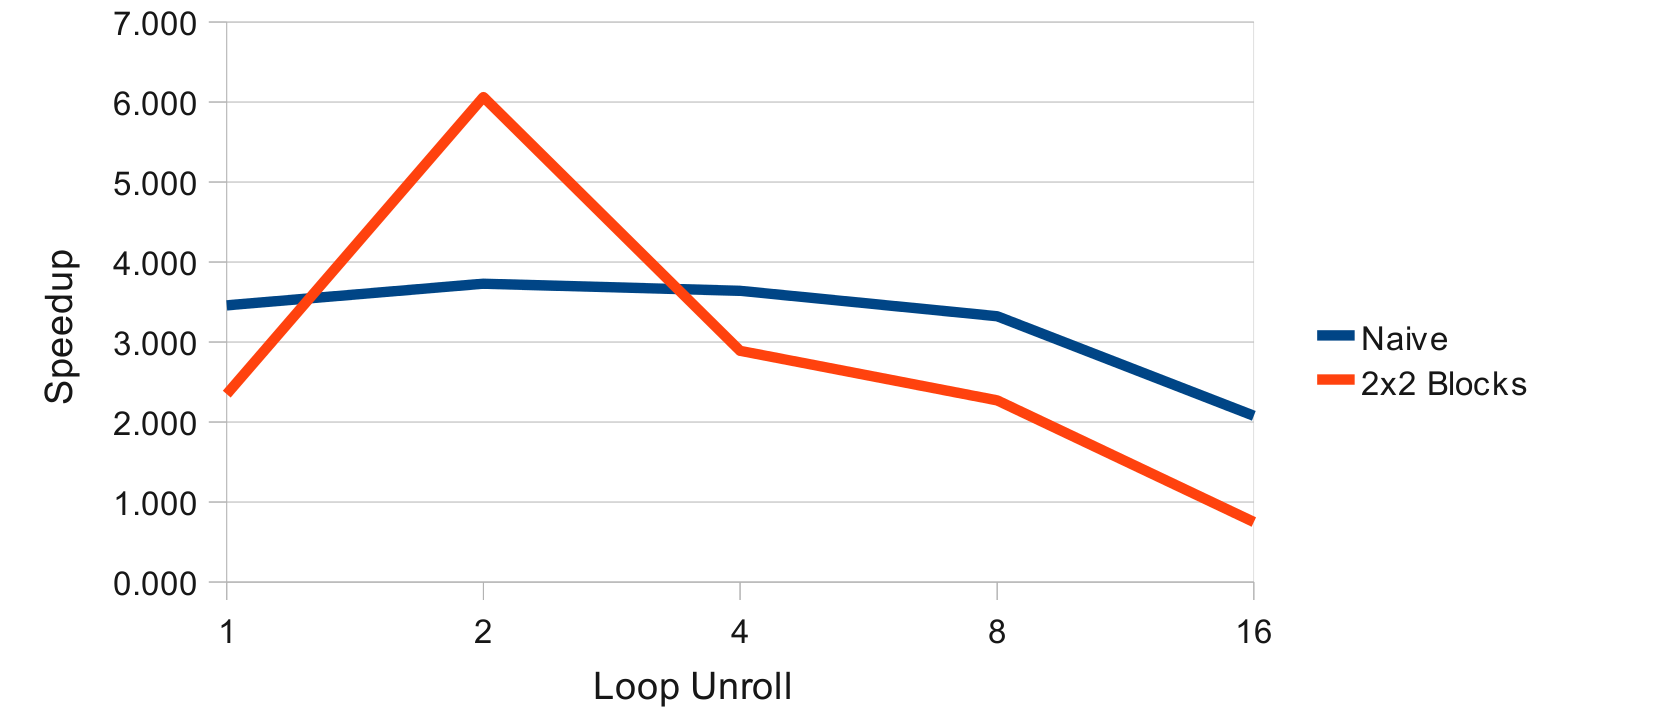
\includegraphics[clip]{unrolling}
\end{center}
\caption{Summary of 4k Matrix Multiplication Performance}\label{unroll}
\end{figure}

\section{Conclusion}

Hai

\bibliography{bacon}{}
\bibliographystyle{splncs03}
\end{document}
